% !TEX encoding = UTF-8 Unicode
%!TEX root = thesis.tex
% !TEX spellcheck = en-US
%%=========================================
\chapter{Experiments and discussion}
\label{chapter:experiments_and_discussion}

Four experiments have been conducted in an attempt to find good ways to use neuroevolution for finding useful mappings from audio features to audio effect parameters. In each experiment, different neuroevolution configurations are compared to find what works better. Due to the random nature of genetic algorithms, results vary from run to run. To deal with this, each configuration gets multiple runs (with different Pseudo Random Number Generator (PRNG) seeds), and results from the runs are aggregated and presented in various figures. Table \ref{tab:experiments_overview} shows a rough overview of the experiments.

\begin{center}
\begin{longtable}{p{2.3cm} p{13cm}}
\caption[Overview of experiments]{Overview of experiments} \label{tab:experiments_overview} \\

\hline \multicolumn{1}{l}{\textbf{Experiment}} & \multicolumn{1}{l}{\textbf{Description}} \\ \hline 
\endfirsthead

\multicolumn{2}{c}%
{{\bfseries \tablename\ \thetable{} -- continued from previous page}} \\
\hline \multicolumn{1}{l}{\textbf{Experiment}} & \multicolumn{1}{l}{\textbf{Description}} \\ \hline 
\endhead

\hline \multicolumn{2}{r}{{Continued on next page}} \\ \hline
\endfoot

\hline \hline
\endlastfoot

\midrule
  1 & Find the best combination of mutation rate and crossover rate \\
\midrule
  2 & Find a good value for structural mutation parameters \\
\midrule
  3 & Compare sets of audio features used in the fitness function. Analyze data from the neuroevolution process. \\
\midrule
  4 & Compare networks of audio effects with individual audio effects. \\
\end{longtable}
\end{center}




\section{General configuration}
Table \ref{tab:general_configuration} shows the parameters used unless otherwise stated in individual experiments

\begin{center}
\begin{longtable}{p{10cm} p{4cm}}
\caption[General experiment configuration]{General experiment configuration} \label{tab:general_configuration} \\

\hline \multicolumn{1}{l}{\textbf{Parameter}} & \multicolumn{1}{l}{\textbf{Value}} \\ \hline 
\endfirsthead

\multicolumn{2}{c}%
{{\bfseries \tablename\ \thetable{} -- continued from previous page}} \\
\hline \multicolumn{1}{l}{\textbf{Parameter}} & \multicolumn{1}{l}{\textbf{Value}} \\ \hline 
\endhead

\hline \multicolumn{2}{r}{{Continued on next page}} \\ \hline
\endfoot

\hline \hline
\endlastfoot

\midrule
  Population size & 20 \\
\midrule
  Add neuron probability & 0.01 \\
\midrule
  Remove neuron probability & 0.01 \\
\midrule
  Add link probability & 0.01 \\
\midrule
  Remove link probability & 0.01 \\
\midrule
  Elite fraction & 0.1 \\
\midrule
  Survival rate & 0.25 \\
\midrule
  Allow clones & Yes \\
\midrule
  Selection method & Tournament selection \\
\midrule
  Hidden activation function & Hyperbolic tangent \\
\midrule
  Output activation function & Sigmoid \\
\midrule
  Effect parameter low-pass filter cutoff frequency & 50 Hz \\
\midrule
  Fitness function & Local similarity \\
\end{longtable}
\end{center}

% !TEX encoding = UTF-8 Unicode
%!TEX root = thesis.tex
% !TEX spellcheck = en-US
%%=========================================
\section{Experiment 1}
In this experiment, the aim is to find good values for crossover rate and mutation rate.

\subsection{Configuration}

\begin{center}
\begin{longtable}{p{5cm} p{7cm}}
\caption[Experiment configuration]{Experiment configuration} \label{tab:exp1_configuration} \\

\hline \multicolumn{1}{l}{\textbf{Parameter}} & \multicolumn{1}{l}{\textbf{Value}} \\ \hline 
\endfirsthead

\multicolumn{2}{c}%
{{\bfseries \tablename\ \thetable{} -- continued from previous page}} \\
\hline \multicolumn{1}{l}{\textbf{Parameter}} & \multicolumn{1}{l}{\textbf{Value}} \\ \hline 
\endhead

\hline \multicolumn{2}{r}{{Continued on next page}} \\ \hline
\endfoot

\hline \hline
\endlastfoot

Number of generations & 20 \\
\midrule
Target sound & Drum loop \\
\midrule
Input sound & White noise \\
\midrule
Effect & Distortion and resonant low-pass filter \\
\midrule
Audio features & mfcc\_0, mfcc\_0\_\_derivative, mfcc\_1 \\
\midrule
Number of runs & 150 per configuration \\
\end{longtable}
\end{center}

\subsection{Results and evaluation}
Figure \ref{fig:exp1_heatmap} shows that one should avoid using a high mutation rate and a low crossover rate. Instead, one of the combinations inside the red region should do well. Bear in mind that the differences between pure yellow and lime green are small in this region, and that these small differences are not statistically significant. The variance could be reduced with more runs, but due to computational time, the number of runs per configuration was limited to 150. The yellow spot is probably a good configuration, albeit not necessarily the best. Muration rate = 0.6 and crossover rate = 0.7 are used in the following experiments.

\begin{figure}[H]
    \centering
    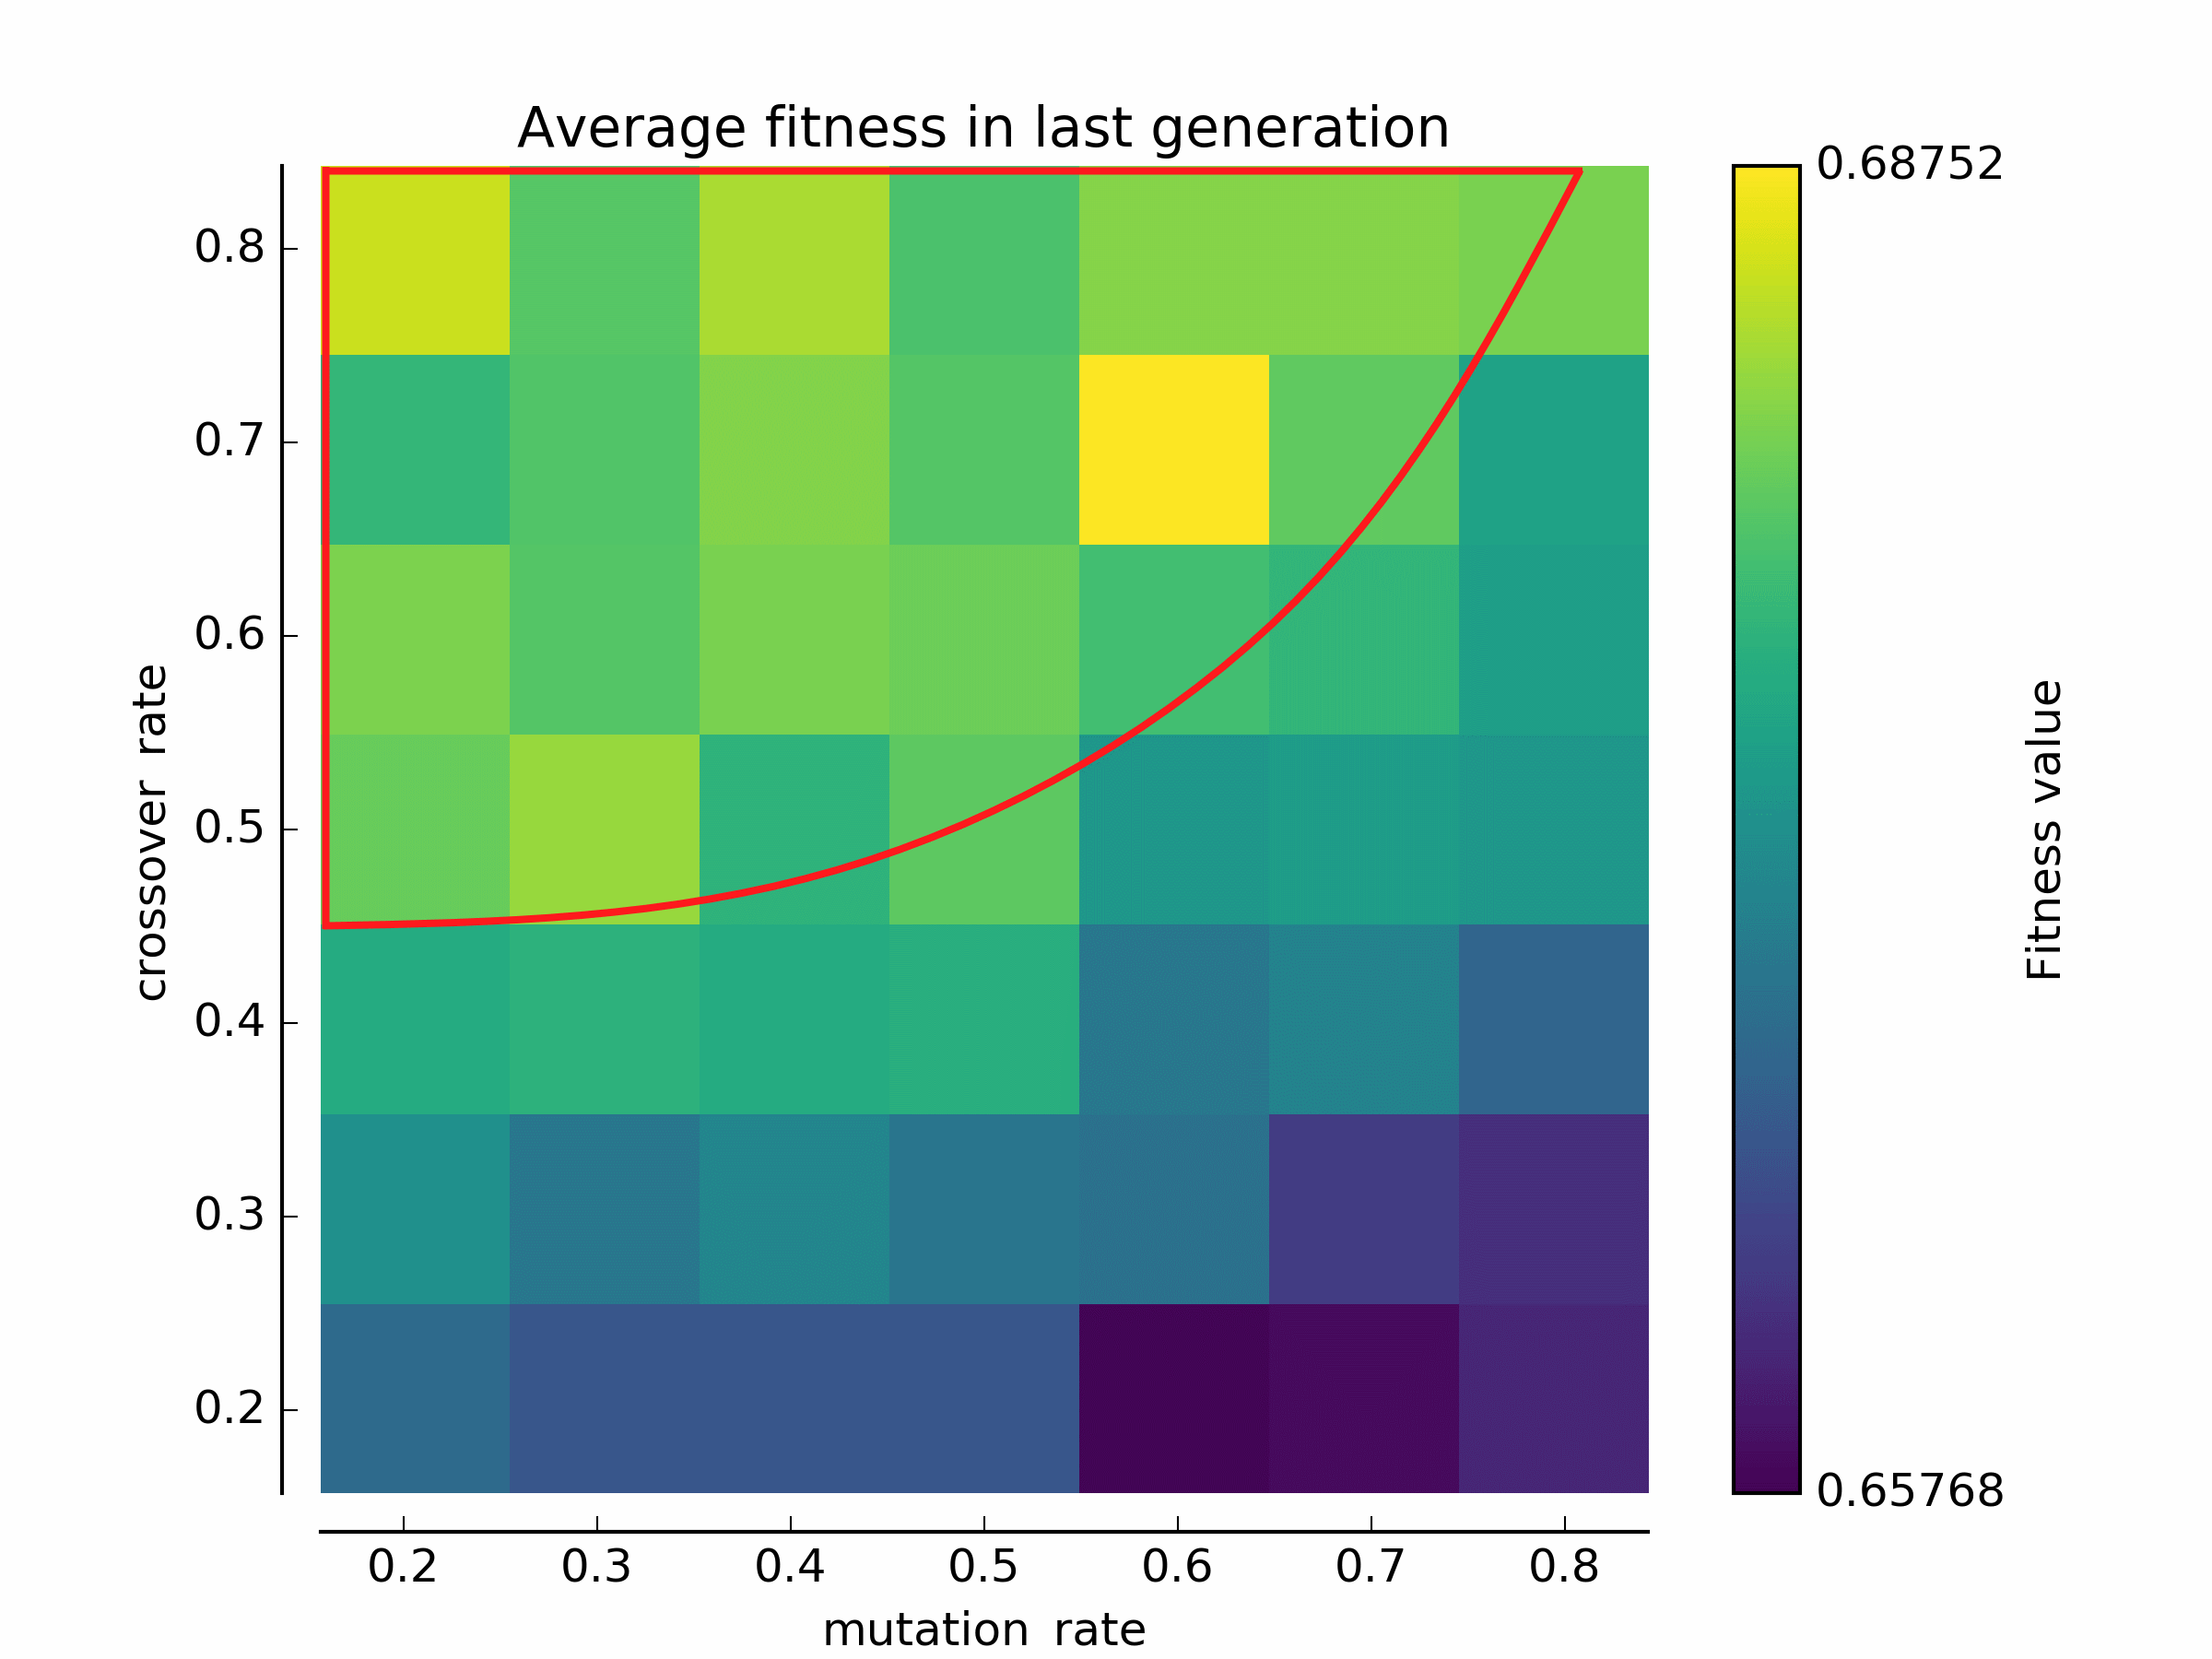
\includegraphics[width=0.99\textwidth]{grid_search_crossover_mutation_avg}
    \caption{The red region drawn on top of the heat map indicates the set of configurations deemed good}
    \label{fig:exp1_heatmap}
\end{figure}
% !TEX encoding = UTF-8 Unicode
%!TEX root = thesis.tex
% !TEX spellcheck = en-US
%%=========================================
\section{Experiment 2}
In this experiment, the aim is to find a good value for add link probability et al TODO

\subsection{Configuration}
\begin{minipage}{\linewidth}
\centering
\captionof{table}{Table Title TODO} \label{tab:title} 
\begin{tabular}{ C{3.5in} C{1.6in} }\toprule[1.5pt]
\bf Parameter & \bf Value \\
\midrule
  Number of generations & 50 \\
\midrule
  Fitness function & Local similarity \\
\midrule
  Target sound & Drum loop \\
\midrule
  Input sound & White noise \\
\midrule
  Effect & Distortion and resonant low-pass filter \\
\midrule
  Audio features & mfcc\_0, mfcc\_0\_\_derivative, mfcc\_1 \\
\midrule
  Number of runs & 400 per configuration \\
\bottomrule[1.25pt]
\end {tabular}\par
\bigskip
Should be a caption TODO
\end{minipage}

\subsection{Fitness function}
Same as in experiment 1

\subsection{Evaluation of configurations}
Figure \ref{fig:add_link_probability} TODO shows that 0.03 is probably the best value while 0.3 is significantly worse

\begin{figure}[h]
    \centering
    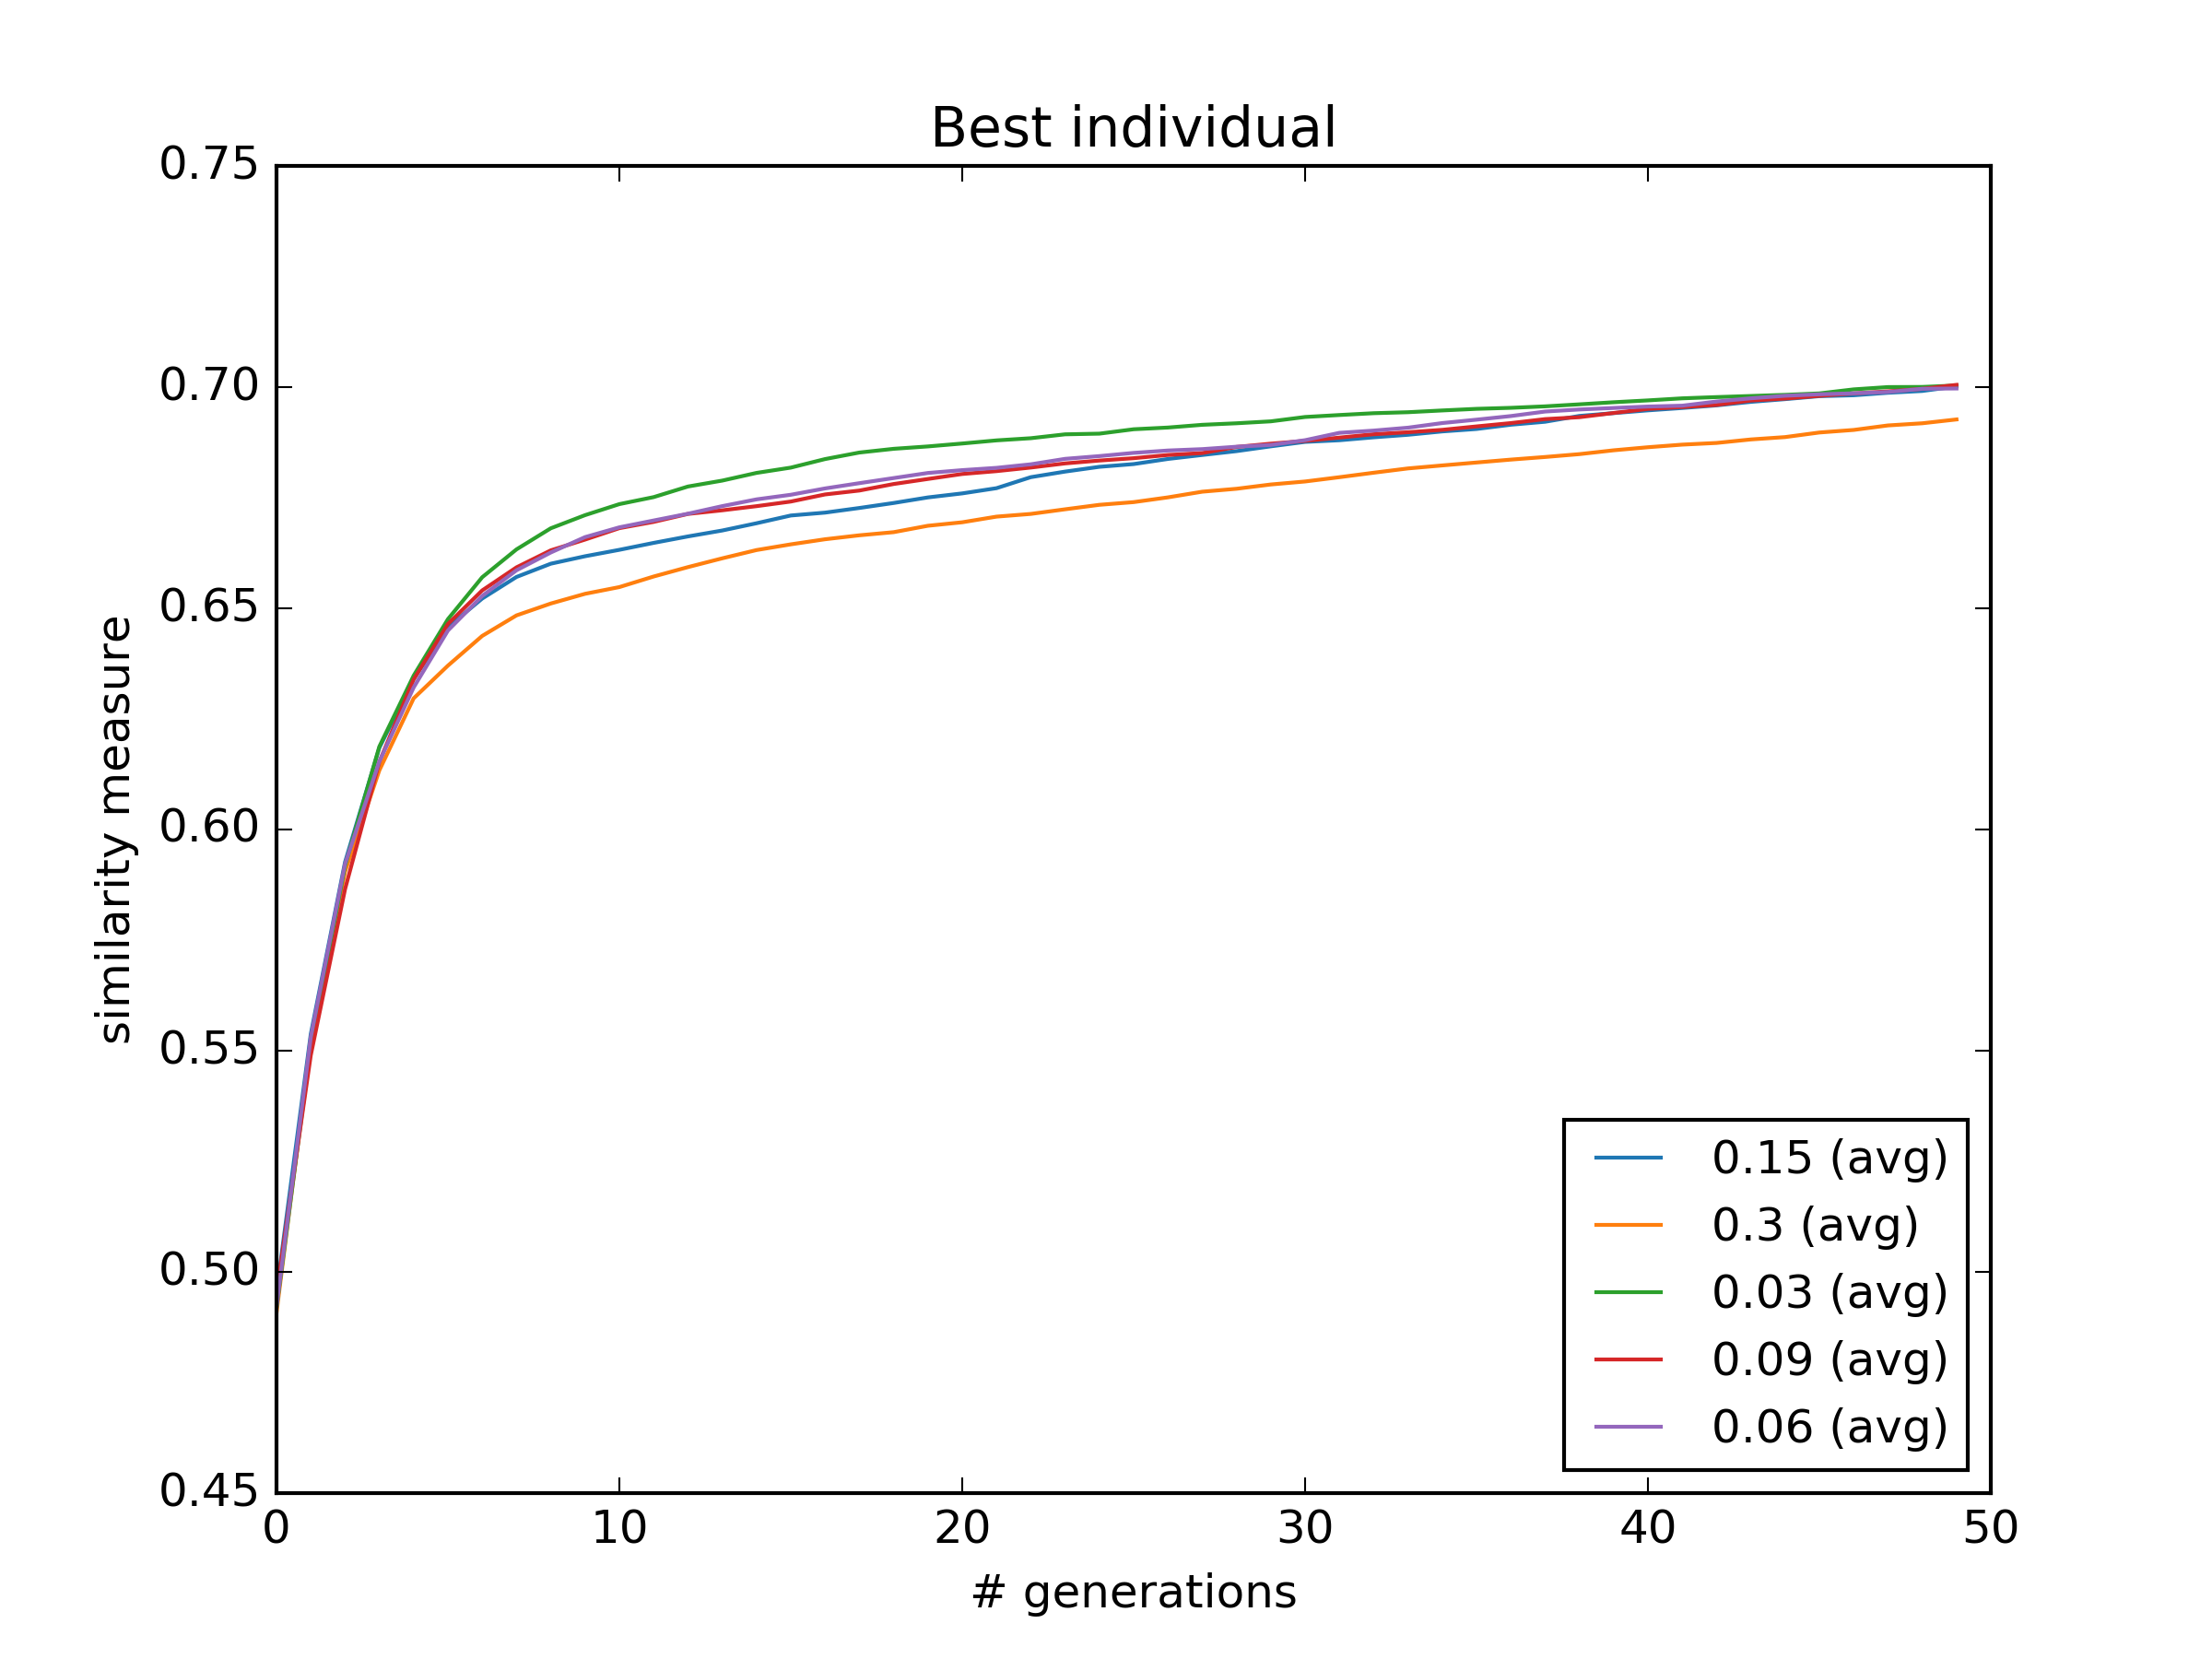
\includegraphics[width=0.99\textwidth]{add_link_probability}
    \caption{TODO caption}
    \label{fig:add_link_probability}
\end{figure}

TODO: Show typical end-result neural networks from all the configurations, to highlight that higher probability builds a larger, more complex network

% !TEX encoding = UTF-8 Unicode
%!TEX root = thesis.tex
% !TEX spellcheck = en-US
%%=========================================
\section{Experiment 3}
When using an evolved cross-adaptive audio effect in a live performance, a performer may want to use it in an expressive way. For example, if the performer is a drummer, he can vary the intensity of the drum hits. For the cross-adaptive audio effect to handle this, it needs to be trained on all the different intensities of the drum hits. If an extensive recording is available, that is fine. However, if the available target sound is short or lacks sufficient variation, one can harness the concept of data augmentation to create artificial variations of that sound. If one uses that sound instead, the evolved effect will typically be more capable of dealing with the generated variations. This experiment is about testing the author's implementation of data augmentation and the ability to apply evolved cross-adaptive audio effects to unseen sounds.

% TODO: mention the sounds and how augmented

\subsection{Configuration}

\begin{center}
\begin{longtable}{p{5cm} p{7cm}}
\caption[Experiment configuration]{Experiment configuration} \label{tab:exp3_configuration} \\

\hline \multicolumn{1}{l}{\textbf{Parameter}} & \multicolumn{1}{l}{\textbf{Value}} \\ \hline 
\endfirsthead

\multicolumn{2}{c}%
{{\bfseries \tablename\ \thetable{} -- continued from previous page}} \\
\hline \multicolumn{1}{l}{\textbf{Parameter}} & \multicolumn{1}{l}{\textbf{Value}} \\ \hline 
\endhead

\hline \multicolumn{2}{r}{{Continued on next page}} \\ \hline
\endfoot

\hline \hline
\endlastfoot

Number of generations & 20 \\
\midrule
Target sound (training) & Drum loop with bass drum, snare drum, clap and hihat (figure \ref{fig:exp3_waveforms}) \\
\midrule
Target sound (validation) & Snare roll (rapid snare drum hits) with ascending pitch and amplitude (figure \ref{fig:exp3_waveforms}) \\
\midrule
Input sound & White noise \\
\midrule
Effect & Distortion and resonant low-pass filter \\
\midrule
Audio features & Root Mean Square (RMS) and spectral centroid \\
\midrule
Number of runs & 40 per configuration \\
\end{longtable}
\end{center}

\begin{figure}[H]
    \centering
    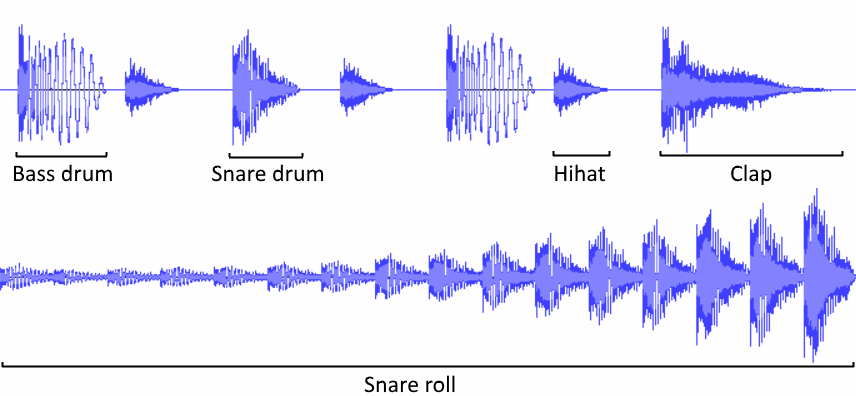
\includegraphics[width=1.0\textwidth]{exp3_waveforms}
    \caption{Waveform of training sound (top) and validation sound (bottom)}
    \label{fig:exp3_waveforms}
\end{figure}

The augmented variant of the training sound was created by repeating the sound 8 times, with variations in playback speed and gain for each repetition. The playback speed and gain are sampled from a gaussian distribution centered around $1$ and with standard deviations of $0.3$ and $0.5$, respectively.

%TODO: mention exponential thingy


\subsection{Results and evaluation}
Figure \ref{fig:exp3_fitness_box} shows that neural networks trained on an augmented variant of the training sound generalizes better than the raw training sound.

% Helps in live settings which typically play in more nuanced ways than the sounds the network is pre-trained on

\begin{figure}[H]
    \centering
    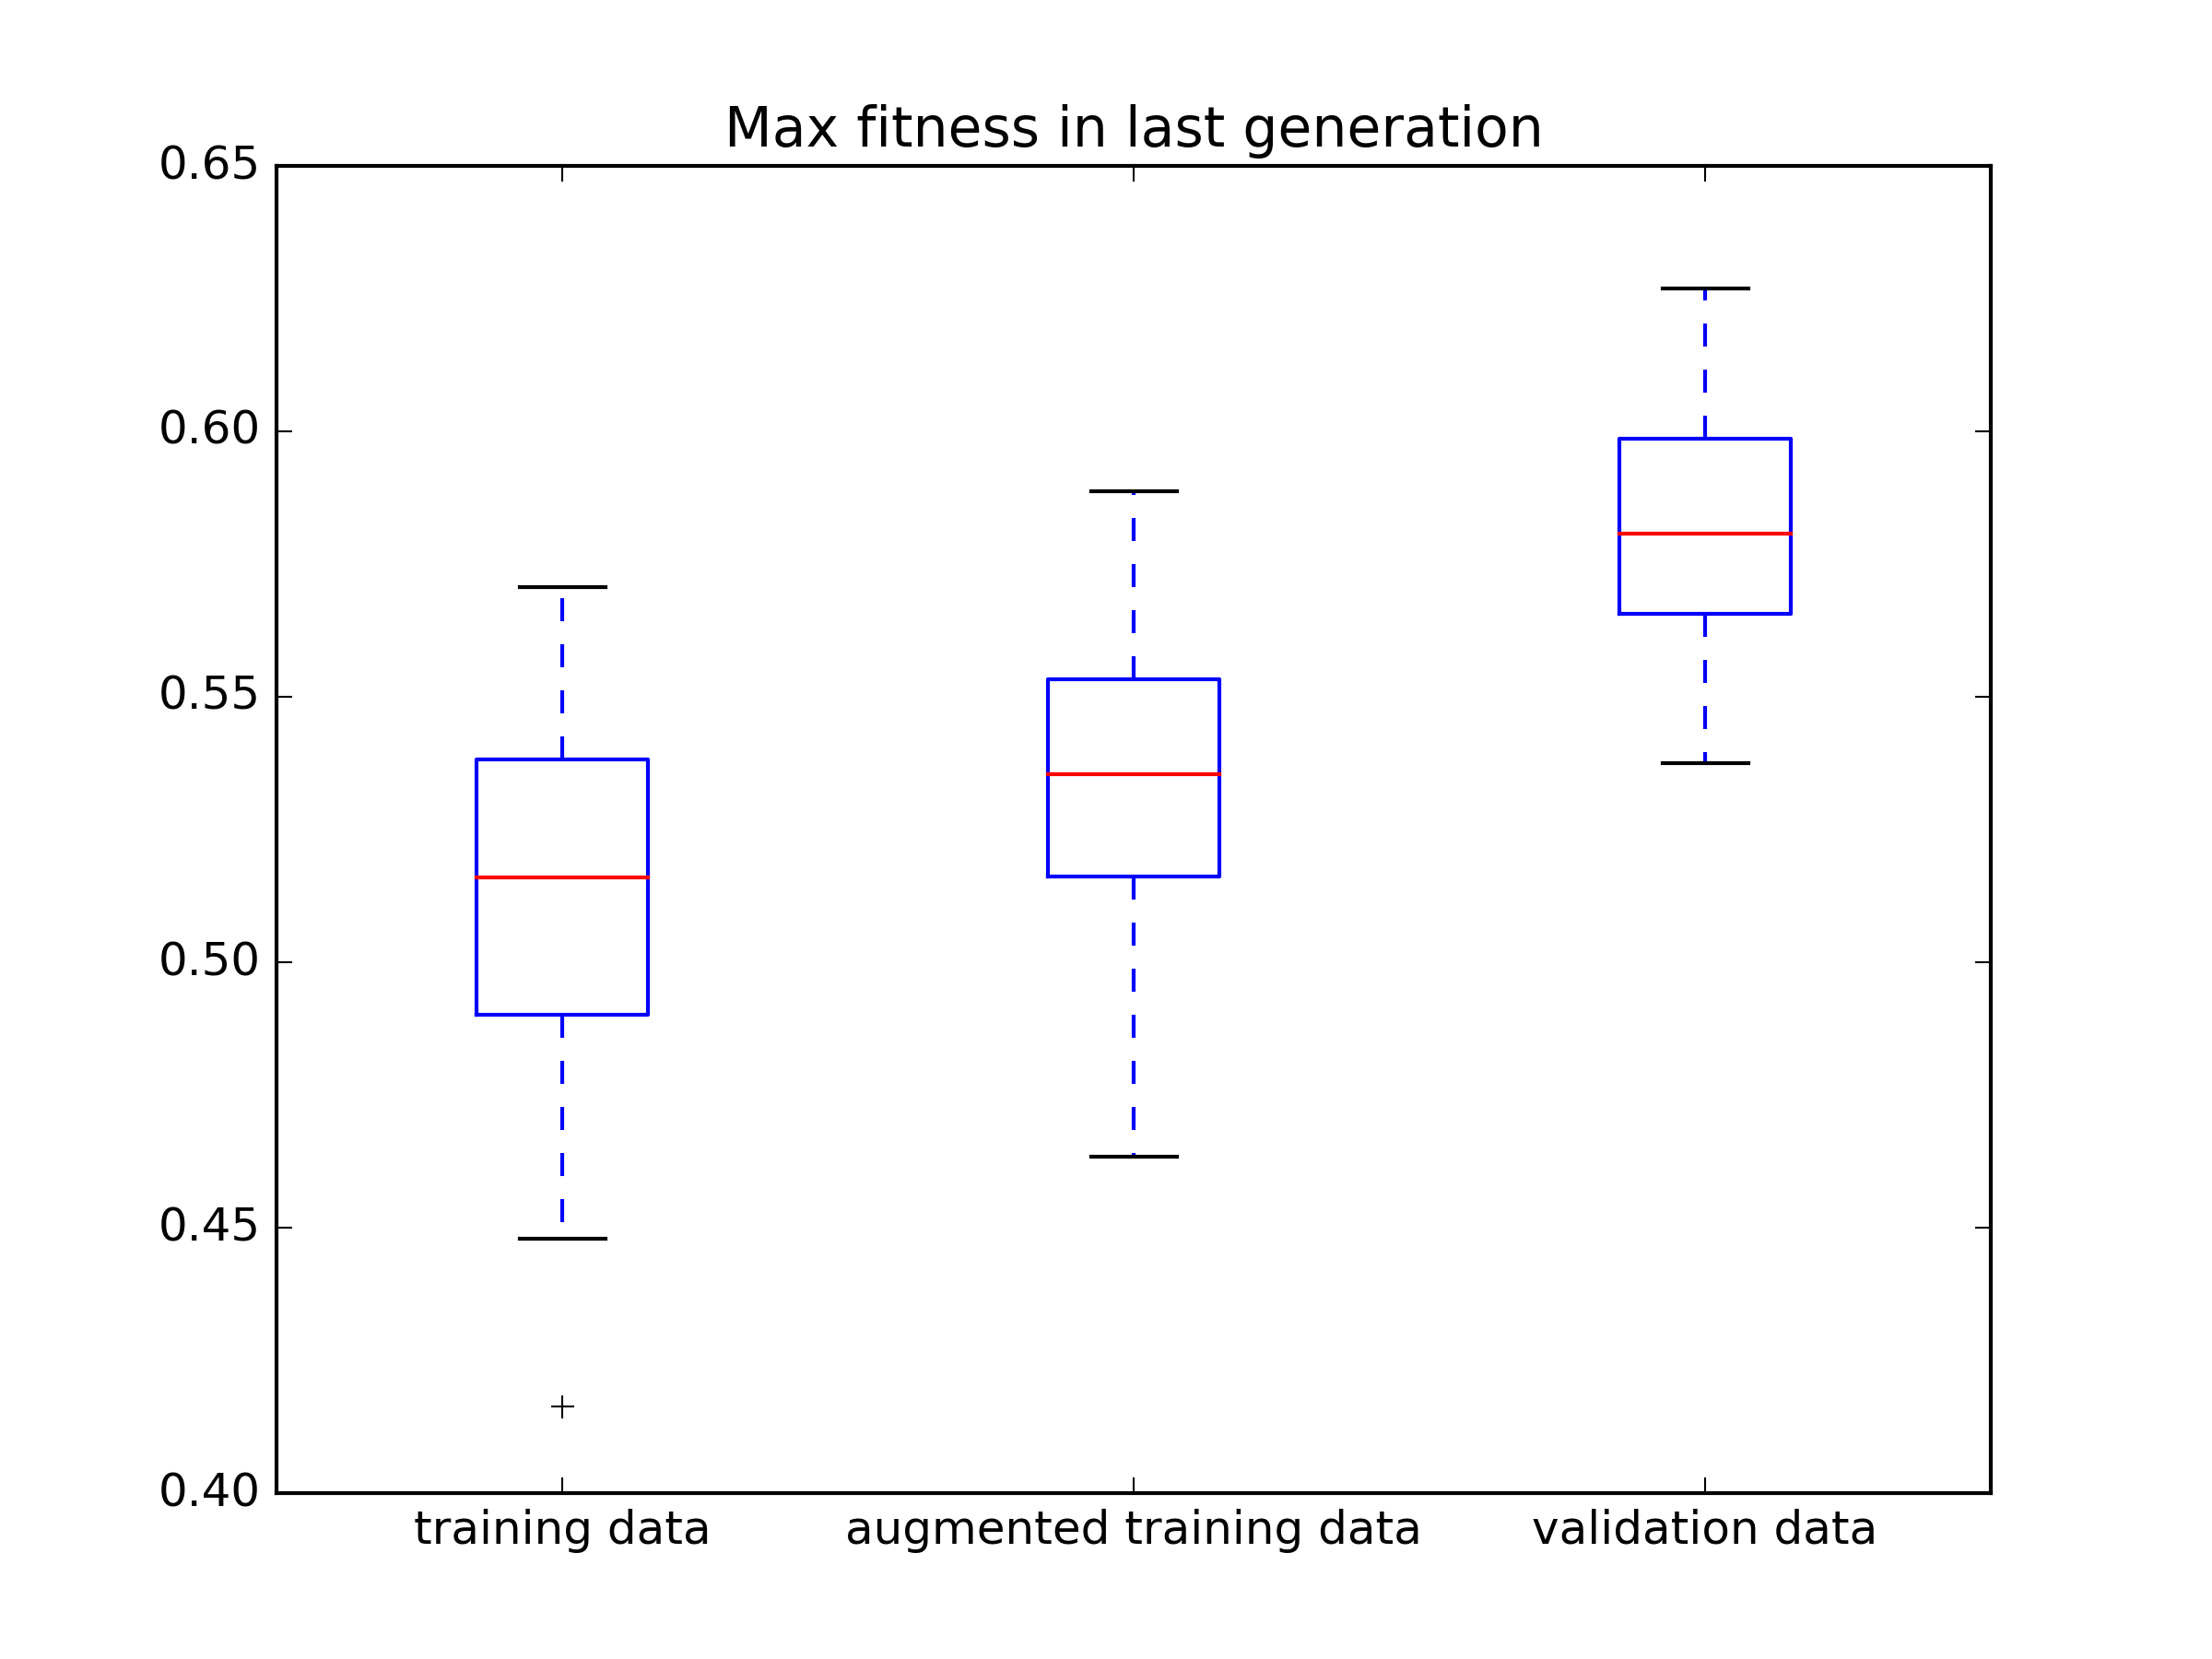
\includegraphics[width=1.0\textwidth]{exp3_fitness_box}
    \caption{Box plot of validation fitness values in final generation. The labels on the x-axis indicate which sound was used as target sound.}
    \label{fig:exp3_fitness_box}
\end{figure}

% !TEX encoding = UTF-8 Unicode
%!TEX root = thesis.tex
% !TEX spellcheck = en-US
%%=========================================
\section{Experiment 3} % TODO: Rename to Experiment 4 if I ever finish and include Experiment 3

\subsection{Configuration}
In this experiment, the aim is to compare two different collections of audio features used in the similarity measure:

\begin{itemize}
\item Configuration A: RMS, pitch and spectral centroid
\item Configuration B: RMS, pitch, spectral centroid and bark bands
\end{itemize}

\begin{center}
\begin{longtable}{p{5cm} p{7cm}}
\caption[Experiment configuration]{Experiment configuration} \label{tab:exp4_configuration} \\

\hline \multicolumn{1}{l}{\textbf{Parameter}} & \multicolumn{1}{l}{\textbf{Value}} \\ \hline 
\endfirsthead

\multicolumn{2}{c}%
{{\bfseries \tablename\ \thetable{} -- continued from previous page}} \\
\hline \multicolumn{1}{l}{\textbf{Parameter}} & \multicolumn{1}{l}{\textbf{Value}} \\ \hline 
\endhead

\hline \multicolumn{2}{r}{{Continued on next page}} \\ \hline
\endfoot

\hline \hline
\endlastfoot

\midrule
Number of generations & 500 \\
\midrule
Target sound & Sine wave, 440 Hz \\
\midrule
Input sound & White noise \\
\midrule
Effect & Band-pass filter with up to 10x post gain \\
\midrule
Number of runs & 20 per configuration \\
\end{longtable}
\end{center}

\subsection{Results and evaluation}
Since fitness functions were different in these two configurations, the fitness values are not directly comparable. Instead, the results were evaluated by manually listening to the output sounds. In the first configuration, the results were fairly bad: All of the sounds were too noisy, and the author failed to perceive the tone. However, in terms of spectral centroid and amplitude, the sounds were a good match. In order to transform noise into a sine, the bandwidth of the band-pass filter has to be very narrow. A narrow filter would have lowered the overall amplitude of the sound. This would have been deemed bad by the fitness function, hence the genetic algorithm did not effectively explore that area in the solution space. Also, a narrow filter would not have yielded any improvements in the similarity in spectral centroid and/or pitch. Therefore, the typical solution has a broad bandpass filter, albeit with an appropriate center frequency. See in figure \ref{fig:exp4_spectrum_plot} that the peak frequency of the typical output sound matches well the peak frequency of the target sound.

The results in the second configuration, were much better. The author could hear a clear tone in all 10 output sounds. There was still some noise in most sounds. The author believes that the solutions would have improved with more generations, because the fitness was typically still increasing towards the 500th (last) generation. One of the output sounds featured vibrato (varying pitch over time), due to a noisy input being mapped to the center frequency parameter. This could probably have been alleviated by adding the derivative of the pitch as a dimension in the fitness function, so the unwanted vibrato would be punished more severely by the fitness function.

\begin{figure}[h]
    \centering
    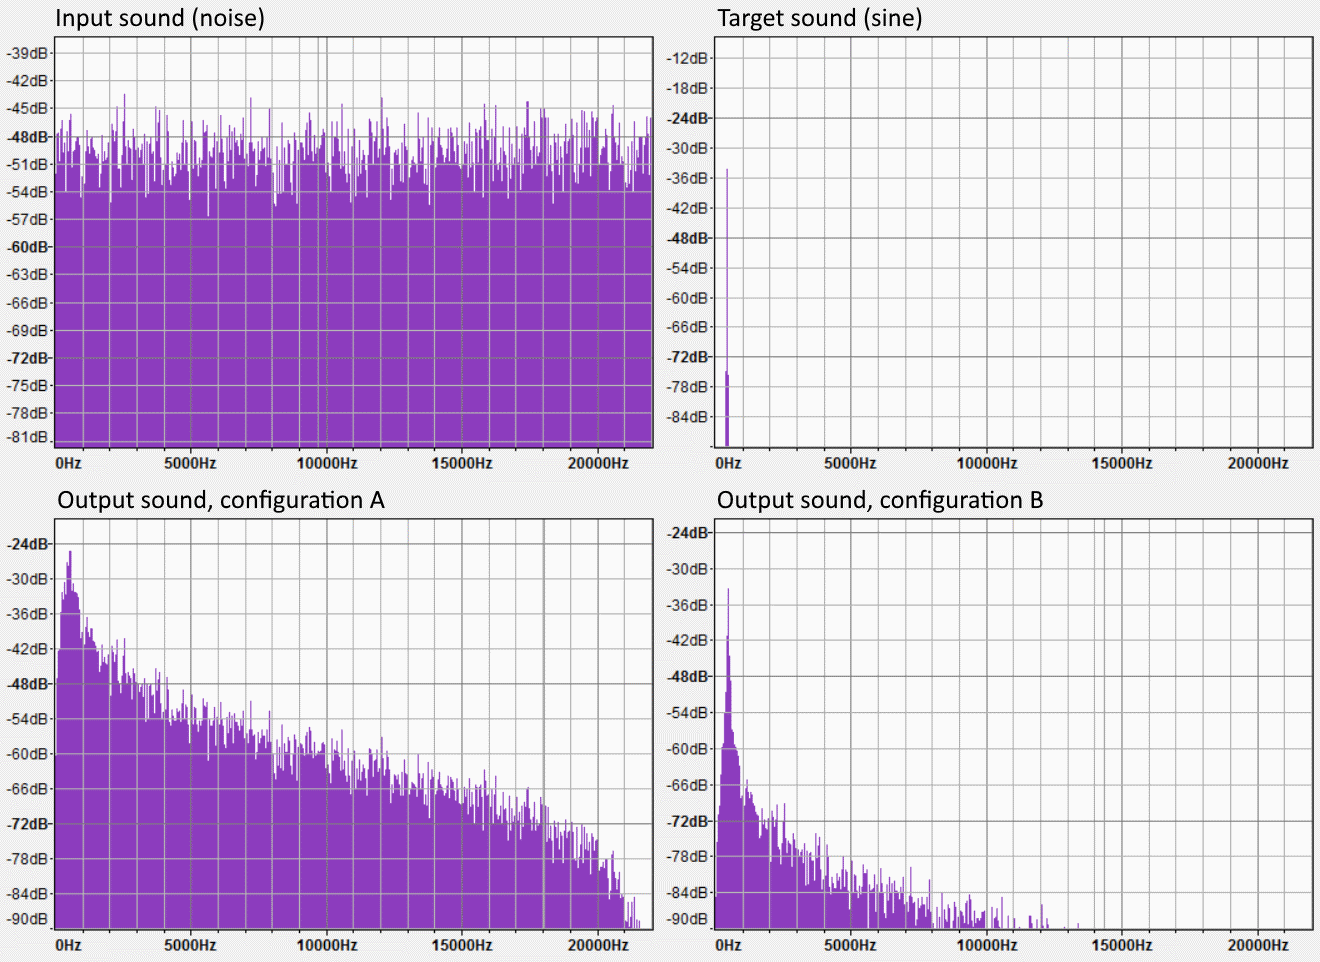
\includegraphics[width=1.0\textwidth]{exp4_spectrum_plot}
    \caption{Spectrum plots, created in Audacity® with hanning window of size 8192}
    \label{fig:exp4_spectrum_plot}
\end{figure}

The takeaway from this experiment is that
\begin{itemize}  
\item the collection of features used for similarity measures has a high impact on the result
\item bark bands are useful
\end{itemize}

\subsection{Neuroevolution analysis}

In this subsection, one of the runs in configuration B will be analyzed, to get a better understanding of how NEAT works in practice, and identify some things that can be improved upon.

In this experiment, the effect parameters do not have to be \textit{dynamically} controlled over time. A static value for each effect parameter (bandwidth, center frequency and post gain) would have been an optimal solution. However, in figure \ref{fig:exp4_typical_nn_evolution}, we see that the NEAT algorithm actually makes use all three input nodes (RMS, pitch and spectral centroid) as well as the constand bias node. The reason for this is that these three inputs do not vary much in the course of the sound, because the features of the sound that was analyzed (sine, 440 Hz) do not vary much over time (see figure \ref{fig:exp4_neural_input}). Consequently, these three nodes act like a bias node with some noise.

\begin{figure}[H]
    \centering
    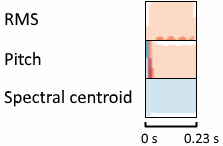
\includegraphics[width=0.3\textwidth]{exp4_neural_input}
    \caption{Neural inputs are almost constant}
    \label{fig:exp4_neural_input}
\end{figure}

\begin{figure}[H]
    \centering
    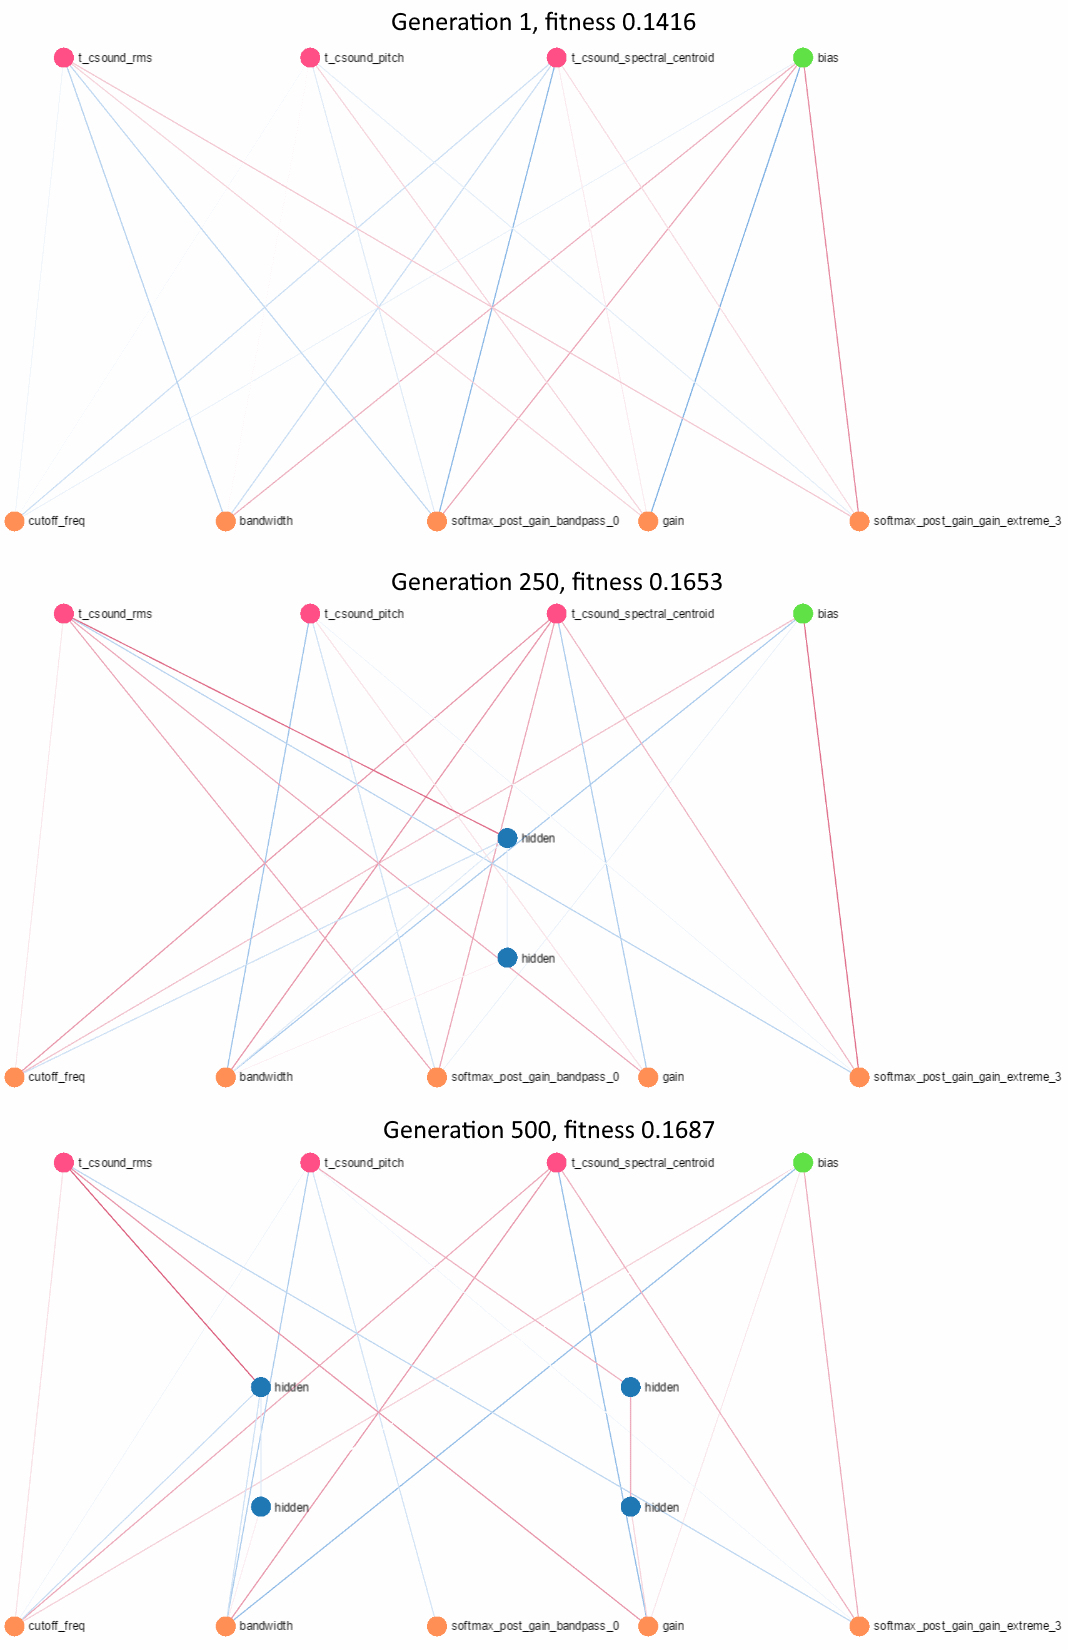
\includegraphics[width=0.9\textwidth]{exp4_typical_nn_evolution}
    \caption{Neural network visualizations}
    \label{fig:exp4_typical_nn_evolution}
\end{figure}

Another interesting fact is that the number of hidden nodes in the best individual tends to increase over the generations, even though these hidden nodes are not needed to get an optimal solution in this experiment. Any constant value can be sent to the output node without having to go through hidden nodes. This is another example of NEAT not finding the optimal solution. Having many hidden nodes hurts evolvability, because an arbitrary mutation on a complex individual is less likely to yield an improvement than the same operation on a simpler individual with fewer hidden nodes. Some form of regularization (punishment for more complex neural networks) could alleviate the problem. Another way to deal with this problem in experiments that do not require hidden nodes is setting AddNodeProbability to zero.

\begin{figure}[H]
    \centering
    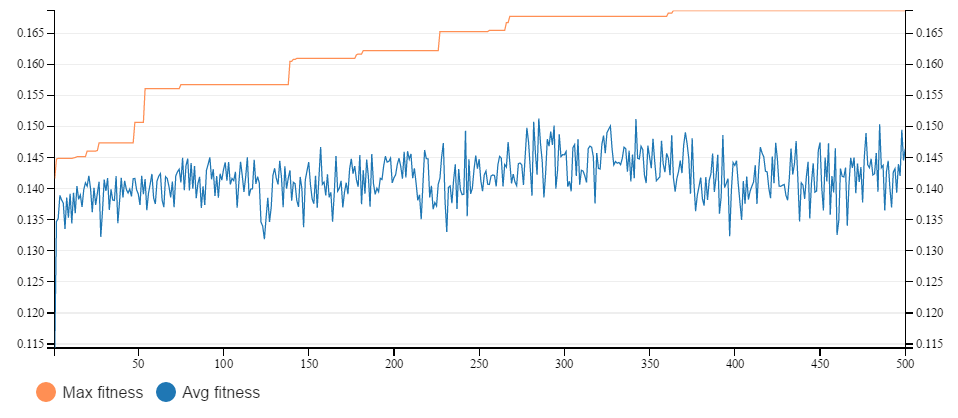
\includegraphics[width=1.0\textwidth]{exp4_fitness_plot}
    \caption{Fitness plot}
    \label{fig:exp4_fitness_plot}
\end{figure}

\begin{figure}[H]
    \centering
    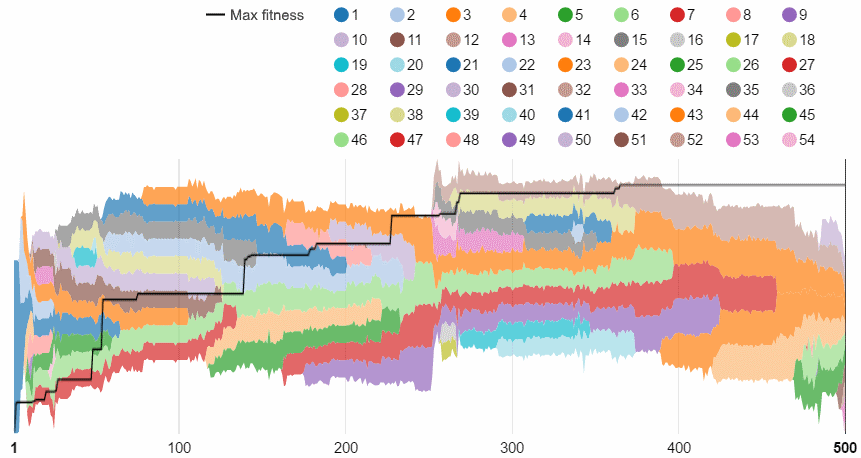
\includegraphics[width=1.0\textwidth]{exp4_species_plot}
    \caption{Species chart with max fitness overlay}
    \label{fig:exp4_species_plot}
\end{figure}

A total of 54 different species were created during the 500 generations of neuroevolution (see figure \ref{fig:exp4_species_plot}). There is no obvious correlation between jumps in max fitness and the death of existing species or the emergence of new species. This makes sense, as competition happens only within species, and species are given time to improve their structure before competition with the rest of the population occurs. The figure also illustrates that the number of species in any given generation is well regulated. The concept of dynamic compatibility threshold in NEAT strives to ensure that the number of species stays within bounds \citep{stanley2004}.

% !TEX encoding = UTF-8 Unicode
%!TEX root = thesis.tex
% !TEX spellcheck = en-US
%%=========================================
\section{Experiment 5}
This experiment is about combining several effects in serial and parallel. The hypothesis is that a genetic algorithm could be adept at choosing which effects to use and how.

For baseline performance measure, each effect has been tested separately. Then they were run in parallel TODO



In this experiment, we do 5 fx in parallel => ok result
am
bandpass
bitreduce
dist lpf
chorus

(Then 2 layers of 5?)
Then 10 fx in parallel => bad result

Suggest pre-training with each fx separately, then training the mix
Softmax mixing may also be bad -> suggest independent mix values

create video demonstrating 1st successful result here

Say something about hypothesis about which fx will be used. Which ones were actually used? Do the same for parameters. Show mix values in horizon graph. Say that am and chorus make sound richer, while we need it filtered.

\begin{figure}[h]
    \centering
    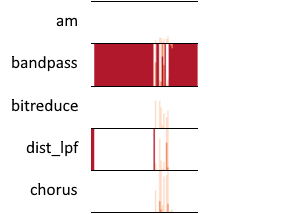
\includegraphics[width=0.45\textwidth]{exp5_1layer_softmax}
    \caption{Gain values for each effect in the best result with configuration 1 TODO}
    \label{fig:exp5_1layer_softmax}
\end{figure}

\begin{figure}[h]
    \centering
    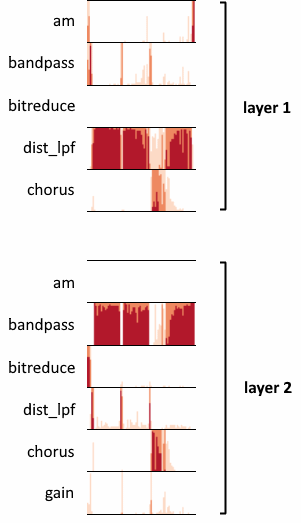
\includegraphics[width=0.45\textwidth]{exp5_2layers_softmax}
    \caption{Gain values for each effect in the best result with configuration 2 TODO}
    \label{fig:exp5_2layers_softmax}
\end{figure}

\begin{figure}[h]
    \centering
    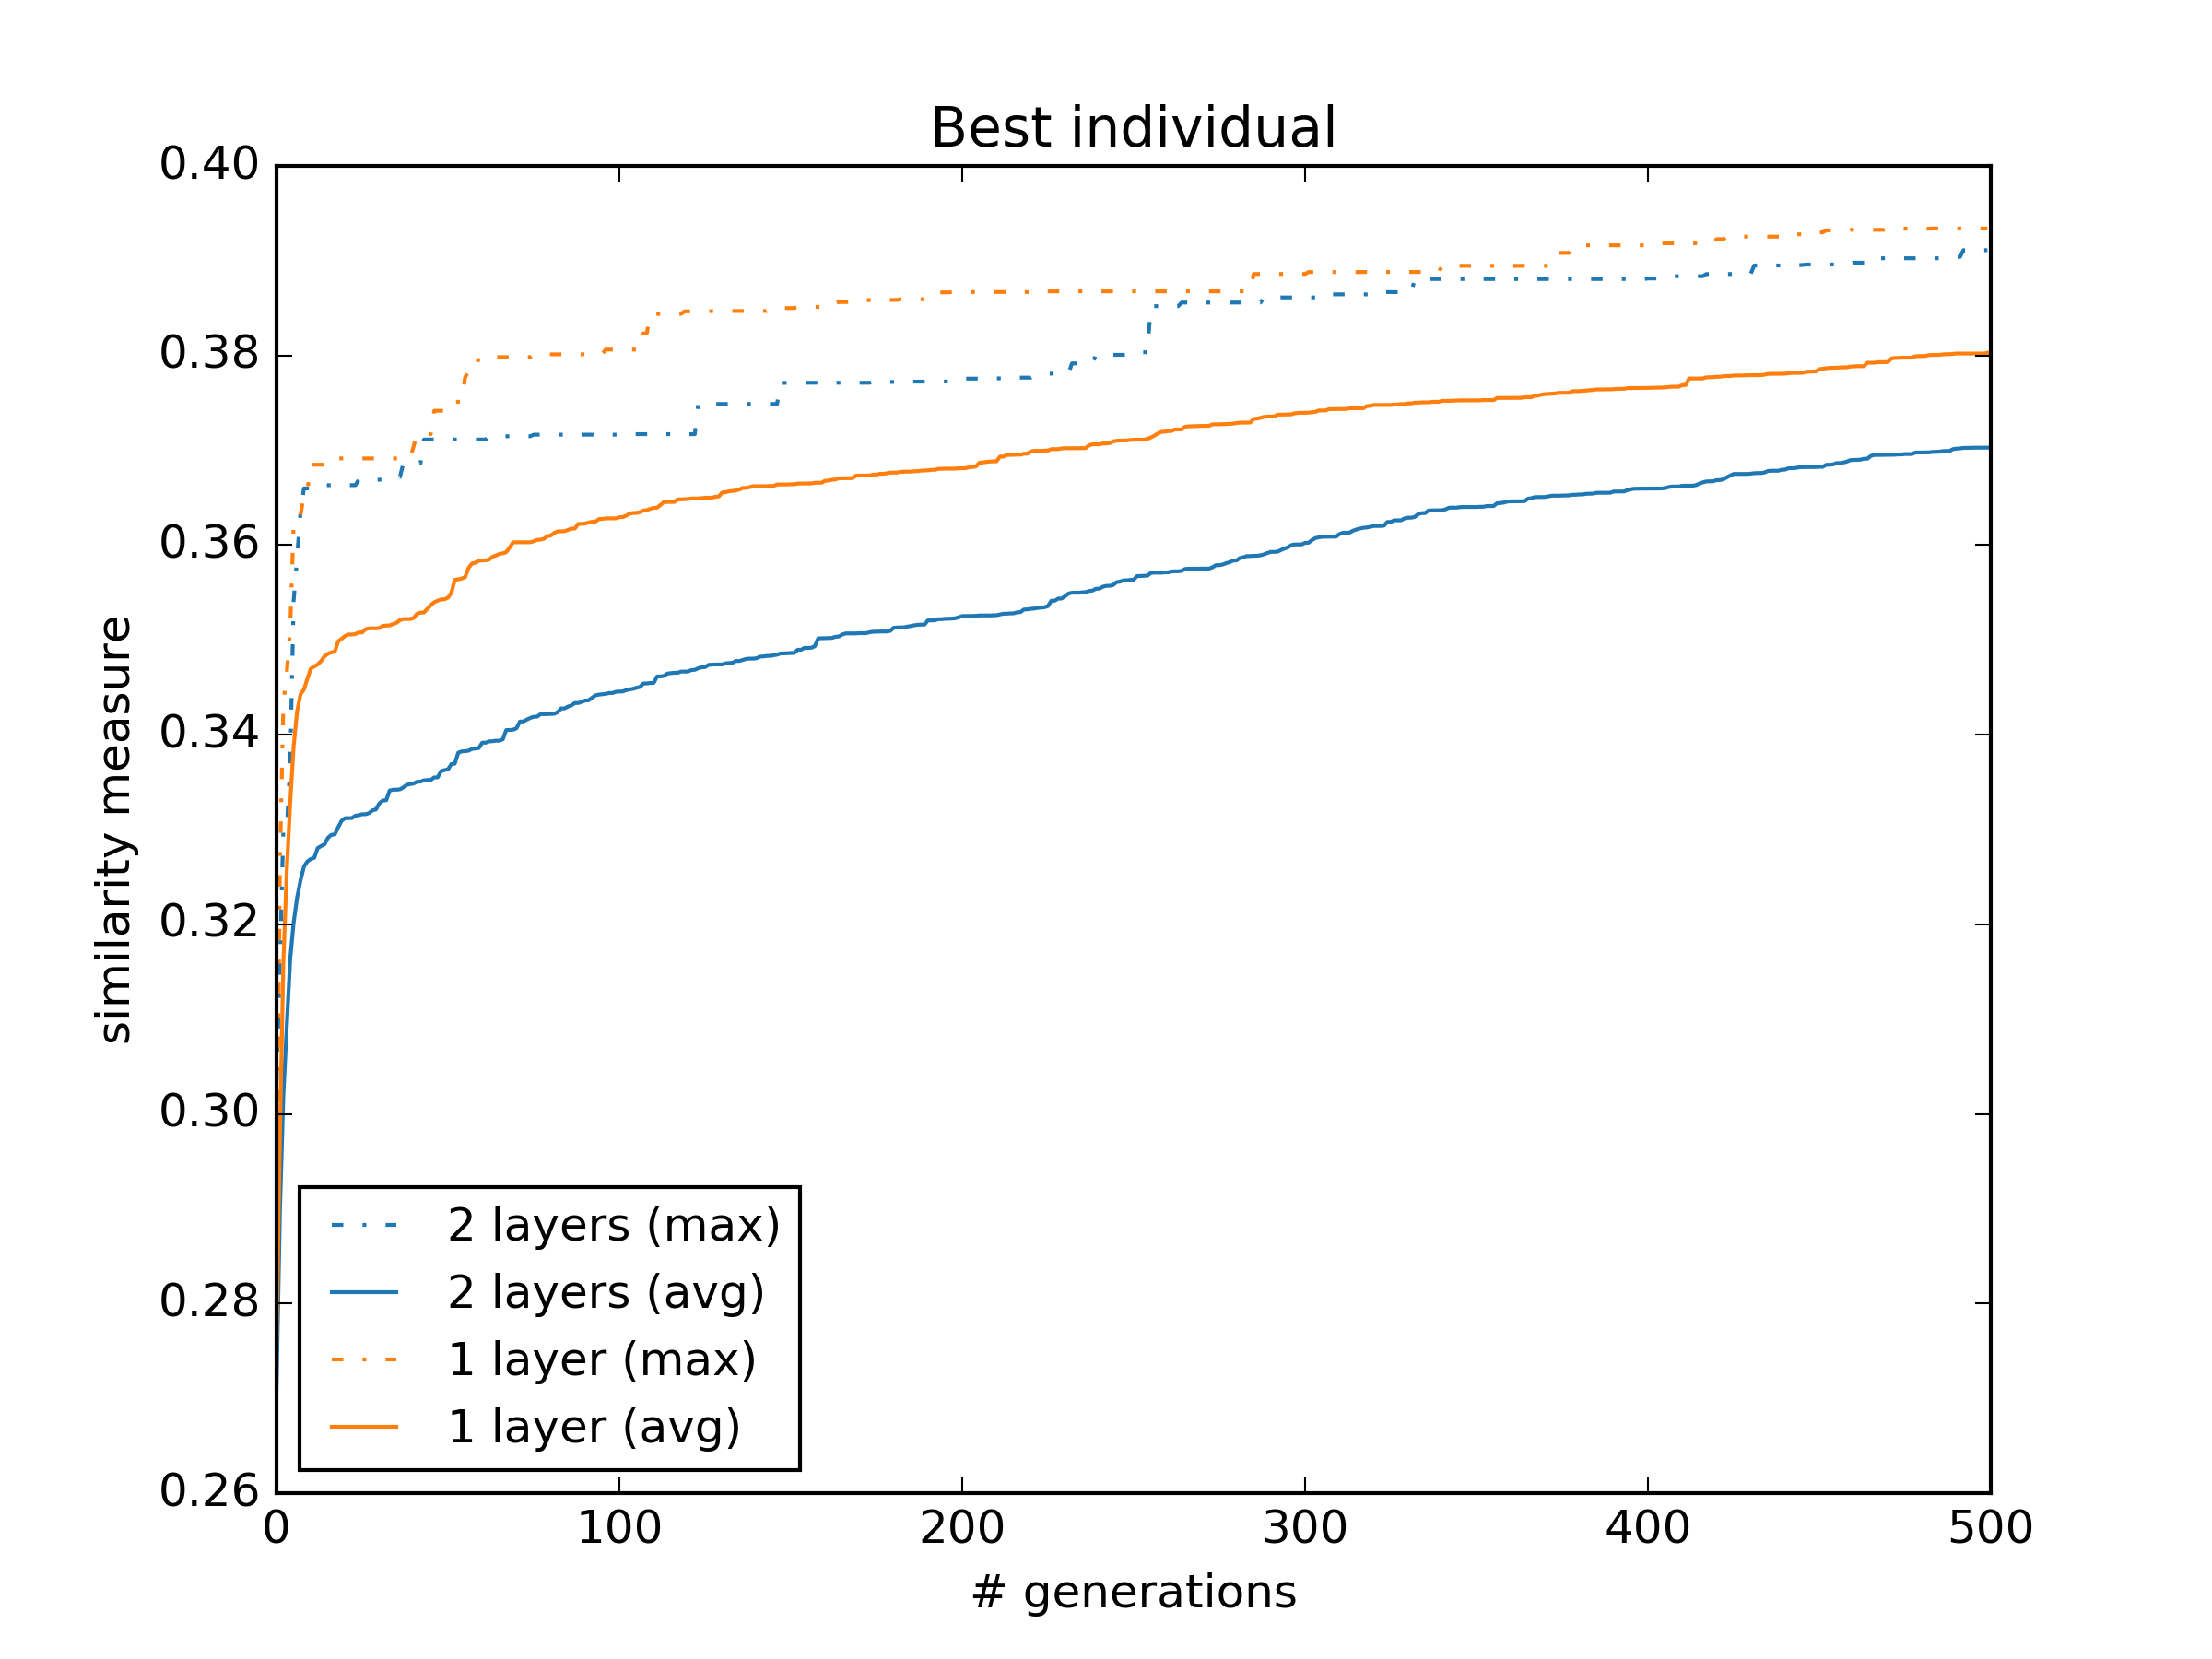
\includegraphics[width=0.99\textwidth]{exp5_avg_max}
    \caption{Aggregated fitness values}
    \label{fig:exp5_avg_max}
\end{figure}

\begin{figure}[h]
    \centering
    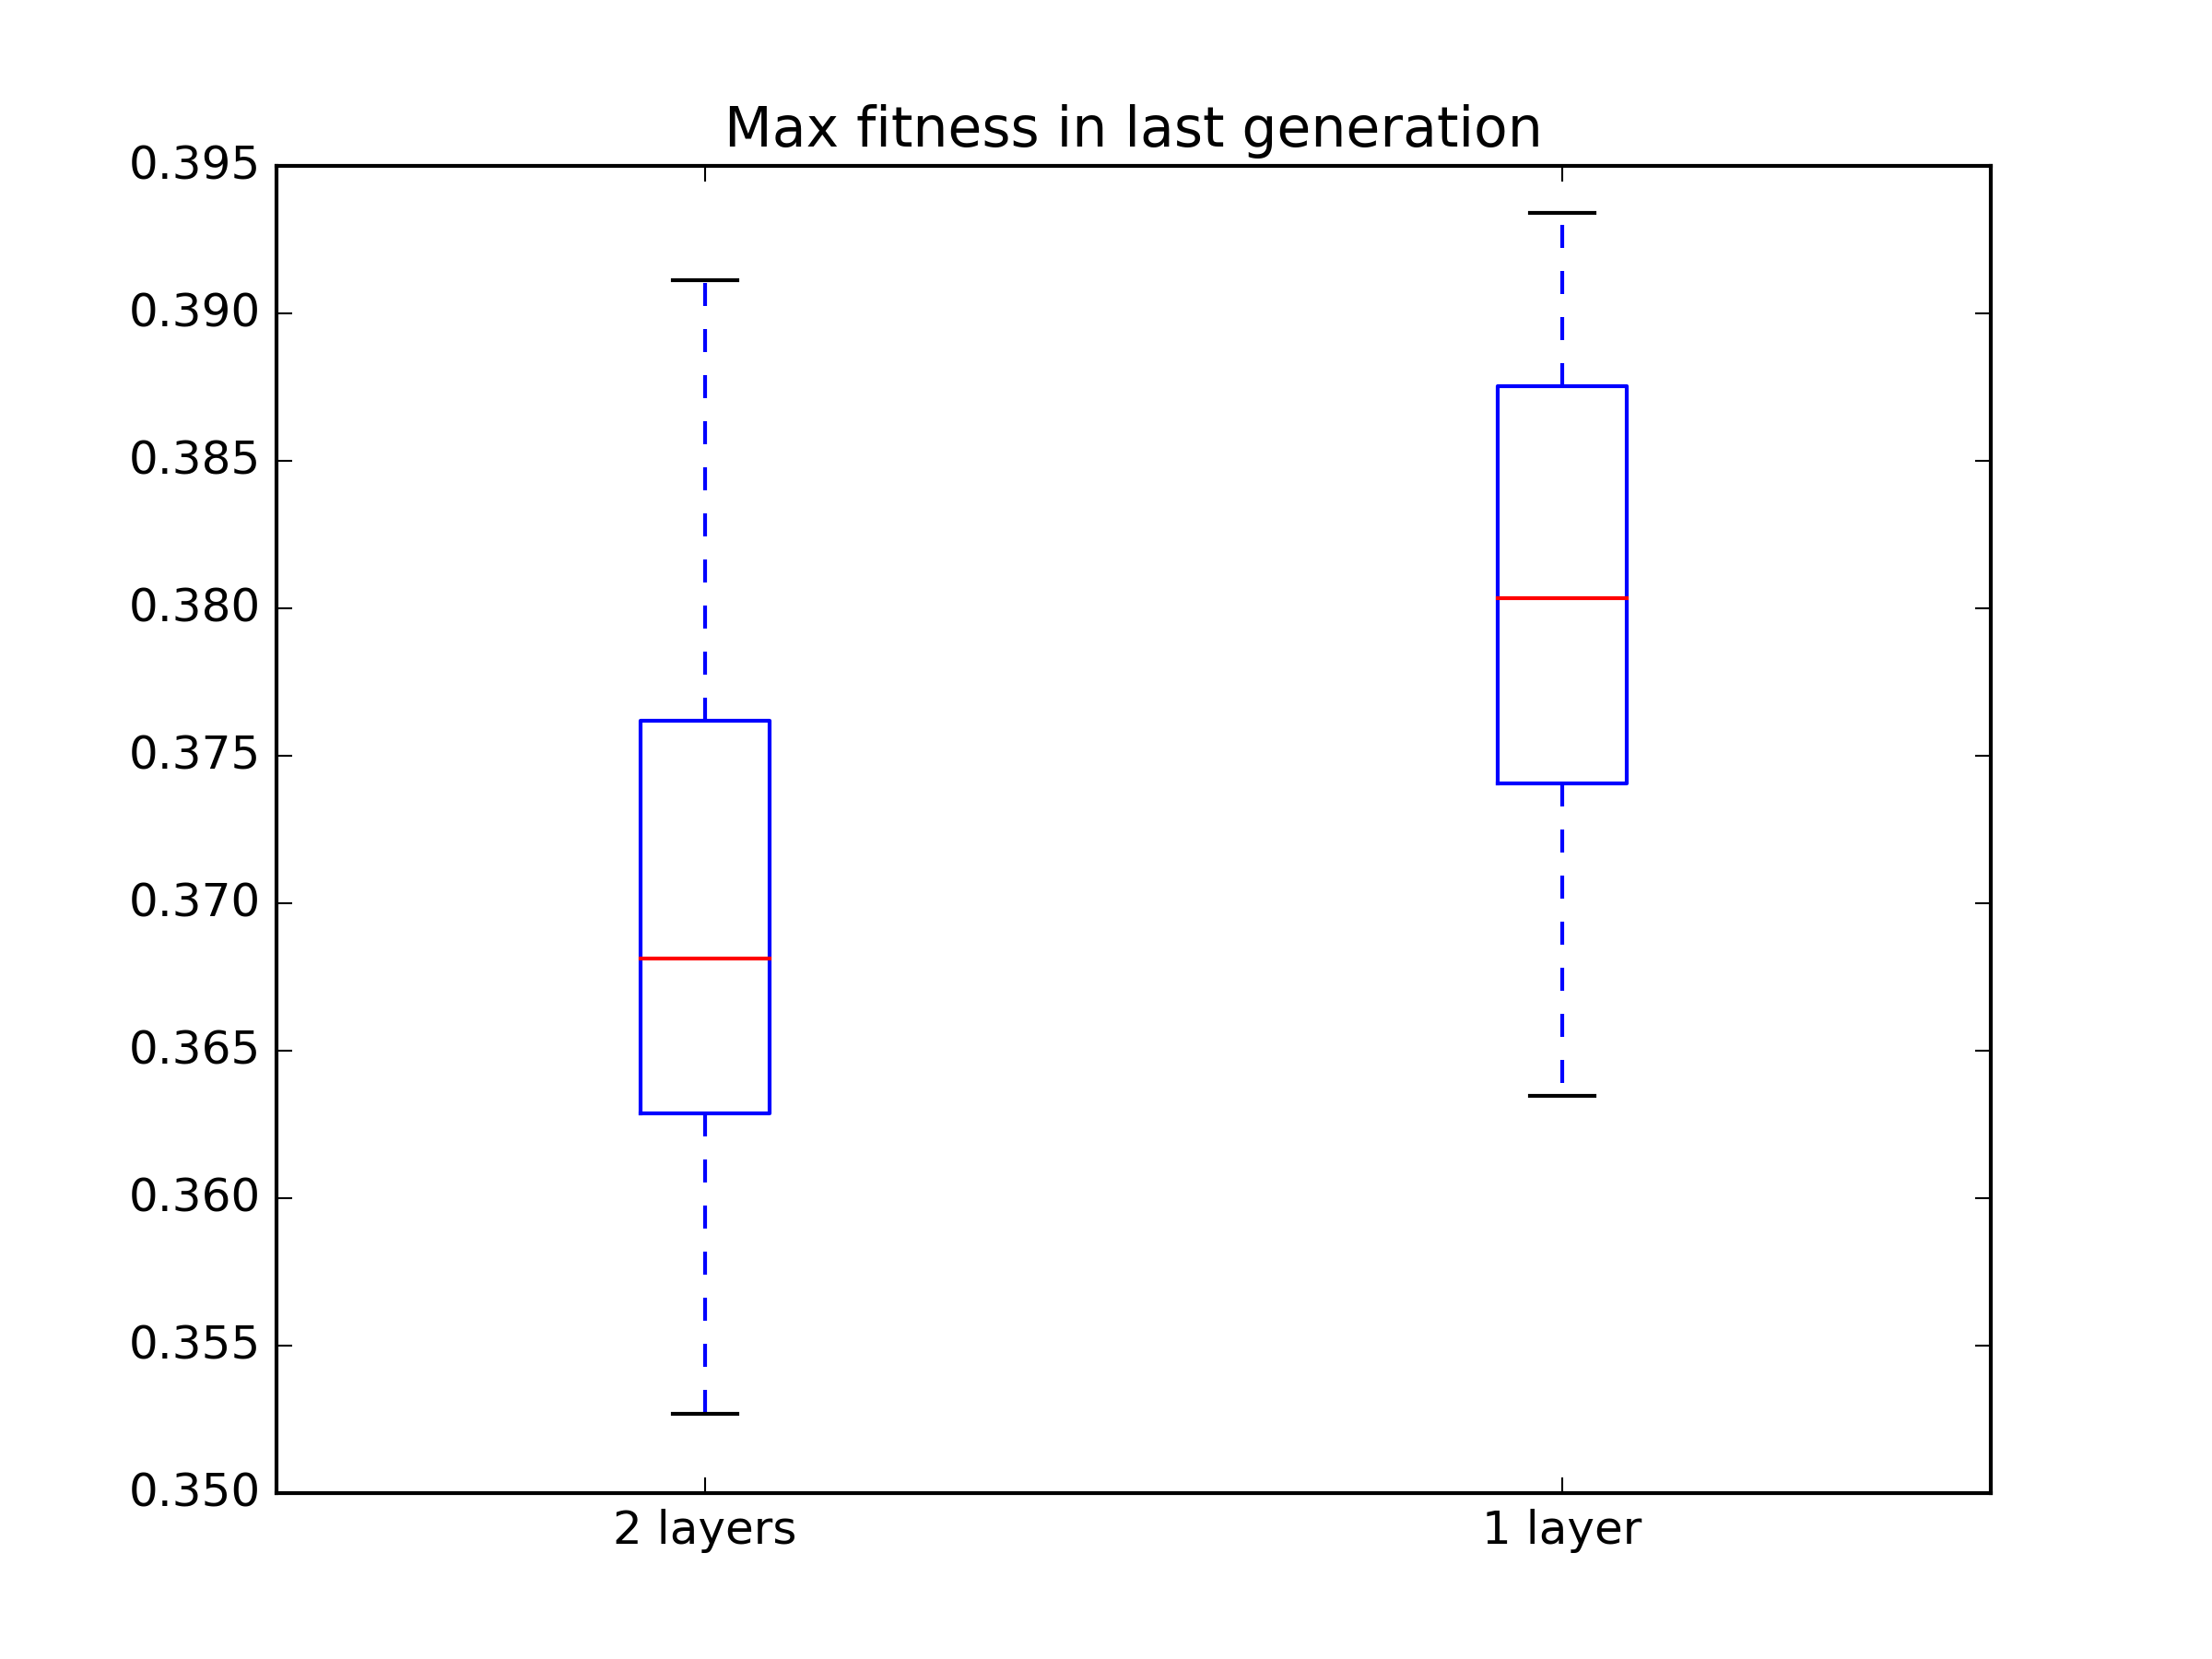
\includegraphics[width=0.99\textwidth]{exp5_box}
    \caption{Box-and-whiskers plot of fitness values in the last generation}
    \label{fig:exp5_box}
\end{figure}

